\subsubsection{AStar (A\*)}
The A* Algorithms is a powerful algorithm used in many games \cite{cai_2015_a}. Like UCS the algorithm uses weighted graph. The A* algorithm is faster than UCS and this is due to a heuristic value that takes notice of the location in relation to the end goal. This heuristic is they key difference between UCS and A* as having this allows A* to select the next node with the lowest cost AND closest to the goal as opposed to just the lowest cost \cite{cai_2015_a}. For this reason, A* will navigate towards the goal as opposed to spanning out from the start point, this in turn leads to A* being the fastest algorithm on this list. Below is a comparison image for the Dijkstra's algorithm vs A* re-enforcing this research and the results found. It can clearly be seen the extra search space from the Dijkstra's, it's also worth noting the implementation of the Dijkstra's algorithm from this source is closer to UCS. 
\begin{center}
	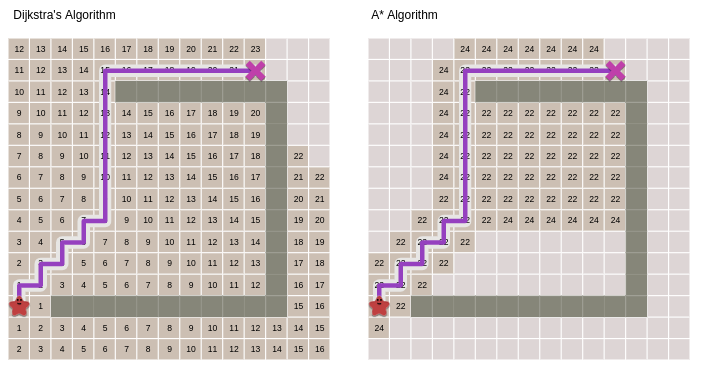
\includegraphics[width=\linewidth]{images/research/Dijkstrasvastar.png}\\
	Visual comparison of UCS vs A* generated from \cite{redblobgames_2014_red}
\end{center}

